\documentclass[11pt,a4paper]{article}
\usepackage[utf8]{inputenc}
\usepackage[T1]{fontenc}
\usepackage{lmodern}
\usepackage[margin=2.4cm]{geometry}
\usepackage{microtype}
\emergencystretch=2em
\usepackage{graphicx}
\usepackage{booktabs}
\usepackage{tabularx}
\usepackage{array}
\usepackage{enumitem}
\usepackage{xcolor}
\usepackage{float}
\usepackage{caption}
\usepackage{amsmath,amssymb}
\usepackage[colorlinks=true,linkcolor=blue!50!black,urlcolor=blue!50!black]{hyperref}
\graphicspath{{../../analysis/figures/paper_sweep/}}
\captionsetup{font=small,labelfont=bf}
\setlist{itemsep=2pt,topsep=4pt}
\newcommand{\code}[1]{\texttt{\small #1}}
\newcommand{\pp}{\,pp}
\newcommand{\rhobar}{\bar{\rho}}
\newcolumntype{L}{>{\raggedright\arraybackslash}X}
\newcommand{\sev}[1]{\textbf{#1}}

\title{\textbf{Interaction-based versus richness-based conservation planning\\ in simulated food webs}\\[4pt]
\large Project summary, critical assessment and proposed article narrative}
\author{Prepared for Diego and collaborators}
\date{16 November 2026 \quad$\cdot$\quad repository branch \code{cleanup/repo-organisation}}

\begin{document}
\maketitle

\begin{abstract}
\noindent This document describes the simulation framework in this repository, how its code is organised
and what it currently shows, and then assesses it with a scientific article in mind. The central
preliminary result is that the \emph{grain of management units} decides whether protecting interactions and
protecting species are aligned or in conflict: with small units an interaction-based plan loses fewer
interactions \emph{and} fewer species than a richness-based plan; with units of one to four home-range
diameters it saves interactions at a small cost in species; with very coarse units the two plans converge.
The result is statistically solid within the explored design, and the code reproduces the stored data
exactly. Its main vulnerabilities are interpretive rather than computational: the regime where the
interaction-based plan wins outright uses management units smaller than a home range, the richness-based
comparator is probably weak at that grain, the primary-extinction rule ignores population size, and the
robustness of the result to the community-assembly parameters has not been tested. Section~\ref{sec:todo}
lists the analyses I consider necessary before submission, in order of priority.
\end{abstract}

\tableofcontents
\newpage

%=====================================================================
\section{The project in brief}

\paragraph{Question.} Conservation planning usually ranks sites by the species they hold. Does ranking
sites by the \emph{biotic interactions} they hold protect ecological networks better, and under which
conditions?

\paragraph{Approach.} A virtual-ecology experiment. A food web is generated, its populations are placed in a
continuous landscape, and energy flowing up from a fixed basal biomass determines which populations can
persist. The landscape is divided into square management tiles. A fixed fraction of tiles is protected
according to one of two rules, populations are then removed at random with a much higher probability
outside protected tiles, and the energetic consequences propagate through the web. The response is the
percentage of species and of species-level interactions lost.

\paragraph{The two strategies compared.}
\begin{description}[leftmargin=1.6cm,style=nextline]
\item[SR] Species richness: protect the tiles holding the most species.
\item[IR] Interaction richness, \emph{egocentric}: protect the tiles whose populations take part in the most
distinct species-level interactions, whether the partner population lies inside the tile or not.
\end{description}
Both are greedy ``top-$k$ by a static tile score'' rules without complementarity. An earlier, tile-internal
definition of interaction richness was discarded because SR outperformed it everywhere.

\paragraph{Status.} The model went through several versions over about two years. The current one (``emergent
assembly'', October 2026) replaced versions whose communities collapsed when stabilised; results from those
versions do not transfer and several reversed. All current results come from one 54,000-run sweep and two
companion runs, all stored in the repository. Funding: BBVA Foundation Leonardo fellowship 2024.

%=====================================================================
\section{Elements of the model}

Table~\ref{tab:elements} lists the components in the order in which a run uses them. The landscape is the
unit square; the median home-range radius is 0.02, so the landscape is 25 median home-range diameters wide.

\begin{table}[!htb]
\caption{Model components (paper configuration).}\label{tab:elements}
\small
\begin{tabularx}{\textwidth}{@{}>{\raggedright\arraybackslash}p{2.6cm}L >{\raggedright\arraybackslash}p{3.8cm}@{}}
\toprule
Component & What it does & Key values \\
\midrule
Metaweb & Niche-model food web; body masses log-normal; a three-level topological class (basal /
intermediate / top) from in- and out-degree. Basal species are herbivores; plants are implicit. &
300 species; connectance $C\in\{0.05,0.1,0.2\}$; $\sigma_{\log M}=1$ \\
Home ranges & Radius $r\propto M^{0.5}$ (area $\propto M$), rescaled to a fixed median. & median $r=0.02$ \\
Range seeding & Each species receives a range fraction $\rho_s=\rhobar\cdot\mathrm{LN}(0,1)$ and
$k_s=\max(1,\mathrm{Poisson}(\rho_s/\pi r_s^2))$ seed populations placed by a Mat\'ern cluster process, so a
species occupies sections of the landscape. & $\rhobar=0.03$; 5 patches per species on average \\
Population web & A metaweb link is realised between two populations when their centres are closer than
$r_\text{pred}+r_\text{prey}$. Links between species that never meet are absent by design. & --- \\
Energetics & Donor-controlled, bottom-up. A fixed basal biomass $B_0$ is split over basal populations. A
consumer population of $n$ individuals needs $n M^{0.75}$; a prey population supplies $\mathrm{TE}\cdot n\,m$,
shared among its predators in proportion to their demand. Population size is the number of individuals the
intake sustains; populations below $n_{\min}$ are removed one at a time, weakest first, and the rest
re-equilibrate. & $B_0=5\times10^6$; TE $=0.1$; $n_{\min}=10$ \\
Management grid & Square tiles; side $t$ in median home-range diameters. &
$t\in\{0.25,0.5,1,2,4,8\}$ $\rightarrow$ $100^2,50^2,25^2,13^2,6^2,3^2$ tiles \\
Protection plan & $\lfloor f\times n_\text{tiles}\rfloor$ tiles with the highest score; ties broken at
random. & budget $f$: 20 values in $0.05$--$0.40$ \\
Primary extinction & One Bernoulli draw per population: probability 0.01 in protected tiles,
$p_\text{ext}$ elsewhere. & $p_\text{ext}\in\{0.3,0.5,0.8\}$ \\
Cascade & The same energetic relaxation, with each population capped at its assembled size. & --- \\
Outcomes & Percentage of species and of species-level interactions lost relative to the stabilised
community, split into primary and secondary, and by trophic group and body-mass quartile. & --- \\
\bottomrule
\end{tabularx}
\end{table}

\paragraph{What the assembled communities look like.} With the paper parameters the stabilised community
holds about 173--191 of the 300 species and 3,600--6,800 populations (Table~\ref{tab:communities}). The
metaweb connectance moves the number of links per species from 3 to 6 while leaving richness almost
unchanged, which is why it was chosen as the web-density axis.

\begin{table}[H]
\centering
\caption{Assembled communities, means over 50 seeds (from \code{paper\_sweep\_summary.txt}).}\label{tab:communities}
\small
\begin{tabular}{@{}lrrrrrr@{}}
\toprule
$C$ & Species & Links/sp. & Realised conn. & Herbivore spp. & Top spp. & Populations \\
\midrule
0.05 & 191 & 3.0 & 0.016 & 19\% & 27\% & 6,807 \\
0.10 & 190 & 4.5 & 0.024 & 11\% & 15\% & 5,124 \\
0.20 & 173 & 6.0 & 0.034 & 5\% & 9\% & 3,552 \\
\bottomrule
\end{tabular}
\end{table}

Two properties of these communities matter for everything that follows. First, herbivore populations are
the large majority of all populations (79\%, 70\% and 63\% for the three connectances; computed from
\code{protected\_sets.csv.gz}), although herbivores are a small minority of species. Second, in the
energetic model basal populations keep their size and never starve, so herbivores can only be lost through
primary extinction.

%=====================================================================
\section{Code logic}

\subsection{One run}
The entry point for the paper is \code{PaperSweep}, which fixes the parameter set
in \code{worldParameters} and calls \code{Observables.runWith}. The flow is:

\begin{enumerate}
\item \textbf{Assemble} (\code{World.assemble}): the metaweb is generated, seed populations are placed,
the population web is built by \code{PopulationWebGenerator}, and the energetic assembly is run by
\code{EnergyFlow.relax}. The result is stored as an \code{Assembly}, together with a snapshot of the
random-number generator.
\item \textbf{Finish} (\code{World.fromAssembly}): lay the management grid for the requested tile size and
build the shared base world. No protection is applied yet.
\item \textbf{Per strategy} (\code{Observables.runStrategy}), on a copy of the base world:
apply the protection plan (\code{ManagementLandscape.applyProtectionPlan}); stabilise; draw primary
extinctions (\code{World.primaryExtinctions}); run the cascade (\code{World.energyFlowCascades});
compute the losses.
\item \textbf{Pairwise metrics}: overlap of the protected tile sets, rank correlation of the two tile
scores, species and interactions covered by each plan.
\end{enumerate}

\paragraph{Pairing.} Both strategies act on the same world, and each strategy's extinction phase is seeded
with the same seed. Reading the code, the random draws are consumed in the same tile and population order
under both strategies, so a population that is unprotected under both plans meets the same fate in both.
The contrast IR $-$ SR is therefore a paired difference with common random numbers, which is why small
differences are detectable with 50 seeds.

\paragraph{Reuse.} The community is assembled once per (connectance, seed) and reused for all 360
combinations of tile size, budget and pressure. \code{ModelChecks} verifies that a reused assembly gives
results identical to a fresh run.

\subsection{Files}
\begin{table}[H]
\small
\begin{tabularx}{\textwidth}{@{}>{\raggedright\arraybackslash}p{5.6cm}L@{}}
\toprule
File(s) in \code{src/main/scala/econetcons/} & Role \\
\midrule
\code{World}, \code{WorldParameters} & Metaweb, seeding, assembly, extinction phases; all parameters \\
\code{EnergyFlow} & Energetic relaxation, foraging rules, flow trophic positions \\
\code{Species}, \code{Population}, \code{PopulationWebGenerator}, \code{Utils}, \code{SquareGrid} &
Traits, placement (Mat\'ern process), spatial realisation of links, grid geometry \\
\code{ManagementLandscape}, \code{ManagementArea}, \code{ConservationStrategy},
\code{ConservationParameters}, \code{TileSelection}, \code{ProtectionStatus} & Tiles, tile scores,
protection plans (12 strategies exist; the paper uses 2) \\
\code{Observables} & Paired outcomes per strategy \\
\code{PaperSweep} & Main sweep; resumable \\
\code{ProtectedSetExport} & Population-level export of protected sets and final webs; can verify itself
against \code{Observables} \\
\code{TrophicLossSweep} & Species loss by flow trophic-position class \\
\code{AssemblyDiagnostic}, \code{WebStructureSweep} & Community diagnostics used for the design decisions \\
\code{ModelChecks} & Consistency checks (energy balance, foraging rules, tiling, reuse equals fresh) \\
\bottomrule
\end{tabularx}
\end{table}

Analysis is in Python, in \code{analysis/paper\_sweep/}. Each script reads from
\code{data/paper\_sweep/} and writes its figures to \code{analysis/figures/paper\_sweep/}. The commands
are tabulated in \code{analysis/README.md}.

\subsection{What I verified}\label{sec:verified}
\begin{itemize}
\item A 32-run sweep with the current code (2 seeds, $C\in\{0.05,0.2\}$, $t\in\{1,4\}$, budgets 0.05 and
0.40, $p_\text{ext}\in\{0.3,0.8\}$) reproduces the corresponding 32 rows of the stored
\code{paper\_sweep.csv} character for character.
\item \code{summary.py} regenerates \code{paper\_sweep\_summary.txt} and the cell-statistics file with no
difference.
\item \code{ModelChecks} passes all its checks.
\item After moving the legacy Scala files out of the build, the same 32-run sweep gives identical rows
and \code{ModelChecks} still passes (Section~\ref{sec:repo}).
\end{itemize}
I did not rerun the full sweep, the population-level export or the trophic-class sweep.

%=====================================================================
\section{Experimental design of the paper sweep}

Full factorial: 3 connectances $\times$ 6 tile sizes $\times$ 20 budgets $\times$ 3 pressures $\times$ 50
seeds $=$ 54,000 runs, each giving a paired SR/IR outcome; no run failed. Two companion data sets were
produced with the same pipeline:
\begin{itemize}
\item a population-level export of what each strategy protects and what survives, at budget 0.15,
$p_\text{ext}=0.8$, $t\in\{0.25,2\}$;
\item species loss by trophic-position class at $t\in\{0.25,0.5,2\}$, $p_\text{ext}=0.8$.
\end{itemize}
Fixed throughout: $\rhobar$, median home range, $B_0$, $n_{\min}$, transfer efficiency, foraging rule, number
of species, and the protected-tile extinction probability (0.01, hard-coded).

\paragraph{Conventions.} Losses are percentages of the stabilised community. Contrasts are IR $-$ SR in
percentage points (pp); negative means IR loses less.

%=====================================================================
\section{Preliminary results}

\subsection{Management grain decides the sign of the species contrast}

\begin{table}[H]
\centering
\caption{Contrast IR $-$ SR by tile size, averaged over connectance, budget and pressure. Standard errors
are computed over the 50 seeds after averaging within seed (my recalculation; see
Section~\ref{sec:stats}). ``Runs'' columns give the share of the 9,000 runs per tile size.}\label{tab:grain}
\small
\begin{tabular}{@{}rrrrrrr@{}}
\toprule
 & \multicolumn{2}{c}{$\Delta$ species (pp)} & \multicolumn{2}{c}{$\Delta$ interactions (pp)} &
 \multicolumn{2}{c}{Runs with IR better on} \\
\cmidrule(lr){2-3}\cmidrule(lr){4-5}\cmidrule(l){6-7}
$t$ & mean & SE & mean & SE & species & interactions \\
\midrule
0.25 & $-1.43$ & 0.13 & $-6.30$ & 0.21 & 52\% (34\% equal) & 69\% (31\% equal) \\
0.5  & $-0.24$ & 0.11 & $-4.39$ & 0.14 & 46\% & 92\% \\
1    & $+0.55$ & 0.06 & $-2.07$ & 0.09 & 30\% & 85\% \\
2    & $+0.79$ & 0.07 & $-0.93$ & 0.06 & 24\% & 70\% \\
4    & $+0.70$ & 0.07 & $-0.57$ & 0.06 & 22\% & 56\% \\
8    & $+0.32$ & 0.07 & $-0.39$ & 0.06 & 11\% (67\% equal) & 24\% (64\% equal) \\
\bottomrule
\end{tabular}
\end{table}

IR loses fewer interactions at every grain, and the saving shrinks steadily as tiles grow. The species
contrast changes sign between $t=0.5$ and $t=1$: IR is better on both counts with the smallest tiles, and
costs between half and one percentage point of species from $t=1$ upwards. At $t=8$ (nine tiles) the plans
are identical in 63\% of runs. Expressed relative to SR's interaction loss, IR's saving falls from 42\% at
$t=0.25$ to 1\% at $t=8$.

The averages hide how large the effect is where it peaks. At $t=0.25$ and $p_\text{ext}=0.8$, the largest
cell means are about $-15$ to $-17$\pp{} of interactions and about $-4$\pp{} of species, at budgets
where SR loses 27--39\% of interactions and 12--19\% of species.

\begin{figure}[H]
\centering
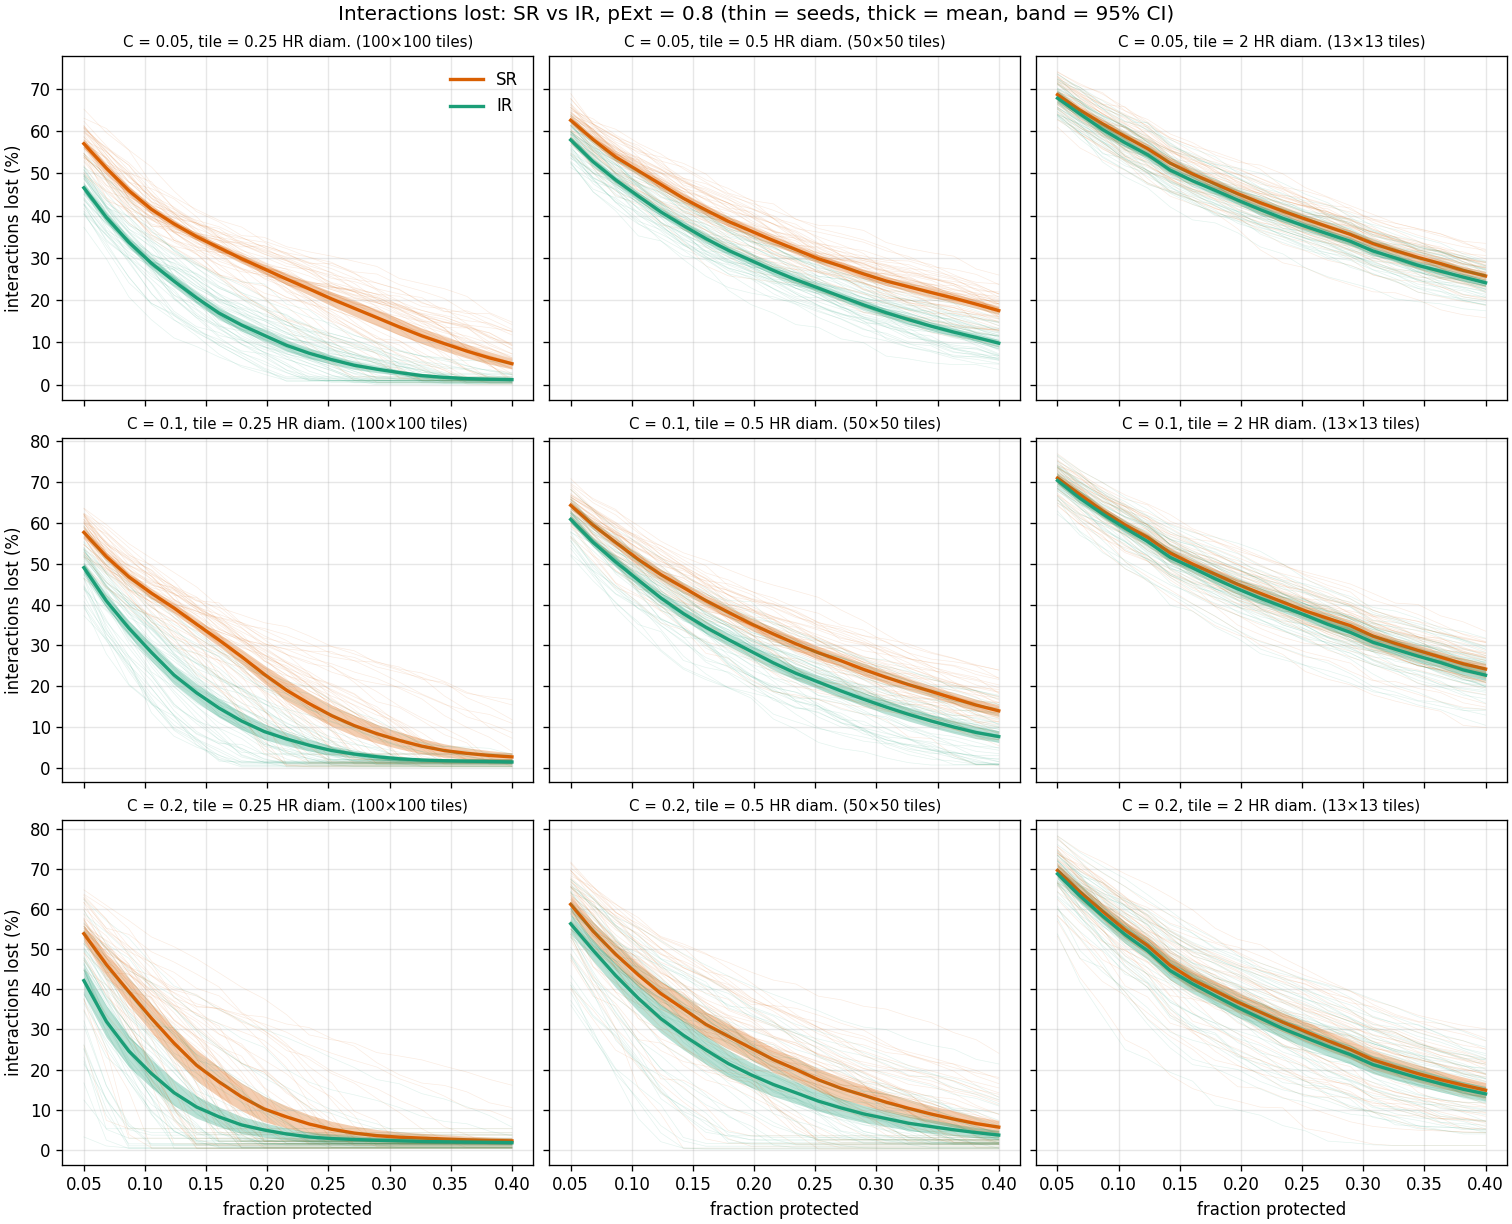
\includegraphics[width=0.92\textwidth]{loss_vs_budget_interactions_pext0.8.png}
\caption{Interactions lost against budget for SR and IR at $p_\text{ext}=0.8$. Rows: metaweb connectance;
columns: tile size 0.25, 0.5 and 2 home-range diameters. Existing figure
(\code{loss\_curves.py}).}\label{fig:curves}
\end{figure}

\begin{figure}[H]
\centering
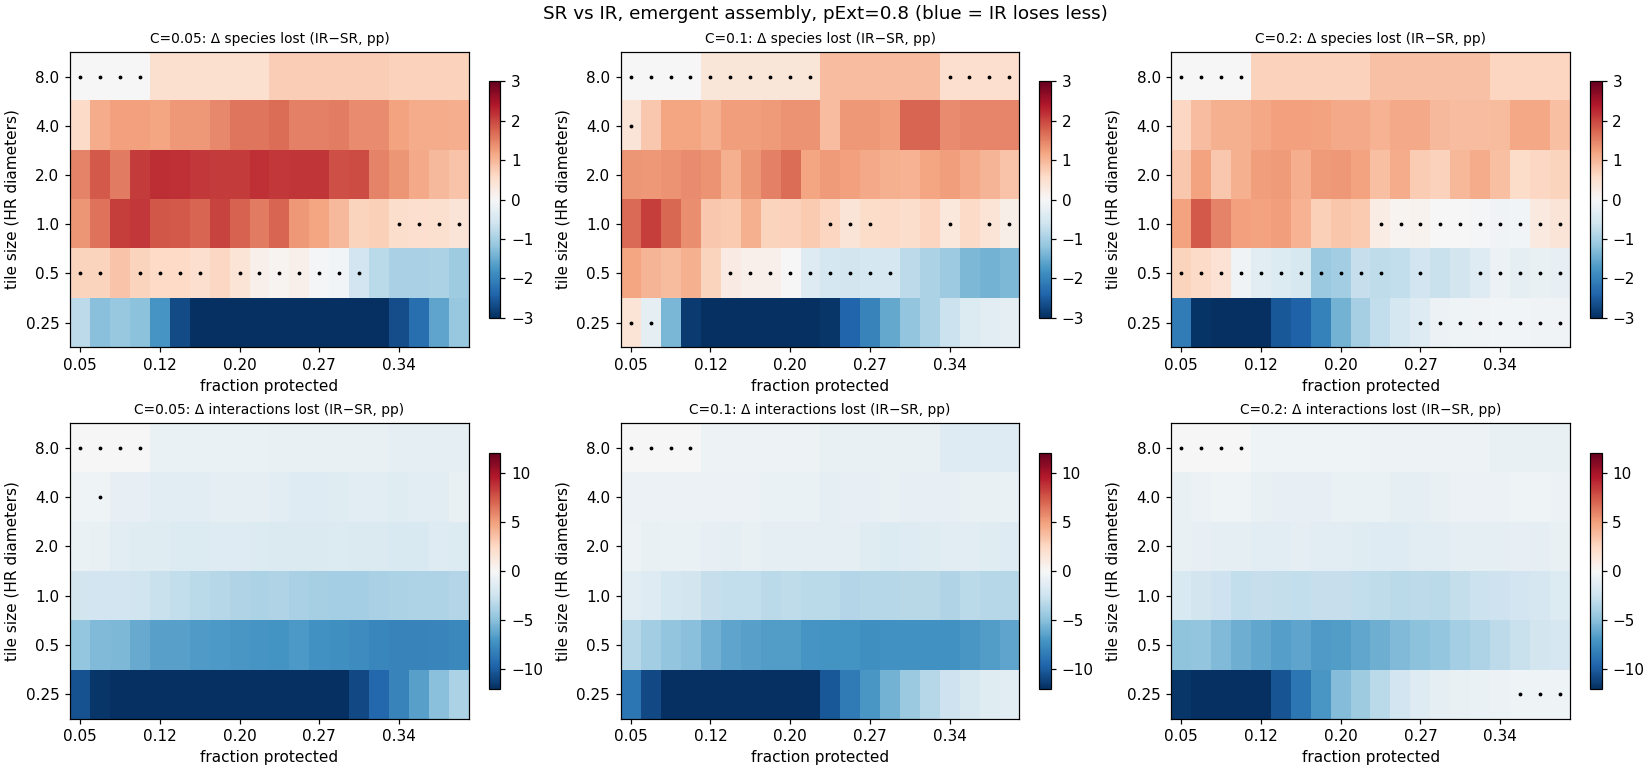
\includegraphics[width=\textwidth]{contrast_heatmap_pext0.8.png}
\caption{Contrast IR $-$ SR over tile size and budget at $p_\text{ext}=0.8$; top row species, bottom row
interactions; blue means IR loses less. Dots mark cells not distinguishable from zero. Existing figure
(\code{heatmaps.py}).}\label{fig:heat}
\end{figure}

\subsection{Pressure amplifies, connectance damps, budget has an interior optimum}
\begin{itemize}
\item Raising $p_\text{ext}$ from 0.3 to 0.8 roughly doubles both contrasts at every grain (for example at
$t=0.25$: interactions $-3.9\rightarrow-8.9$\pp, species $-0.9\rightarrow-2.1$\pp).
\item Denser webs reduce IR's interaction advantage (at $t=0.25$: $-8.2$\pp{} at $C=0.05$, $-4.2$\pp{} at
$C=0.2$).
\item At the finest grain the advantage peaks at budgets of roughly 12--25\% and vanishes above about 30\%,
where both strategies lose almost nothing (Figure~\ref{fig:curves}, left column).
\end{itemize}

\subsection{The plans differ, and they differ in which populations they protect}
The two protected tile sets are substantially different: Jaccard dissimilarity of roughly 0.45--0.72 at a 5\%
budget, decreasing with budget and with connectance. Yet at budget 0.15 both plans cover nearly the same
\emph{species}. What differs is the set of \emph{populations} (Table~\ref{tab:pops}).

\begin{table}[H]
\centering
\caption{Share of baseline populations inside protected tiles at budget 0.15, means over 50 seeds (my
calculation from \code{protected\_sets.csv.gz}).}\label{tab:pops}
\small
\begin{tabular}{@{}llrrrr@{}}
\toprule
$t$ & $C$ & Strategy & All populations & Herbivore populations & Consumer populations \\
\midrule
0.25 & 0.05 & SR & 53\% & 51\% & 60\% \\
     &      & IR & 45\% & 38\% & 72\% \\
0.25 & 0.10 & SR & 61\% & 59\% & 68\% \\
     &      & IR & 56\% & 45\% & 81\% \\
0.25 & 0.20 & SR & 81\% & 79\% & 85\% \\
     &      & IR & 71\% & 58\% & 93\% \\
\midrule
2 & 0.05 & SR & 27\% & 26\% & 30\% \\
  &      & IR & 25\% & 24\% & 29\% \\
2 & 0.20 & SR & 42\% & 40\% & 48\% \\
  &      & IR & 41\% & 37\% & 47\% \\
\bottomrule
\end{tabular}
\end{table}

With fine tiles, IR protects \emph{fewer} populations than SR in total but markedly more consumer
populations. With tiles of two home-range diameters the two plans protect almost the same mix. This is the
most direct mechanistic statement the data support: at fine grain the interaction criterion moves
protection up the food web, away from the numerically dominant herbivore populations.

Table~\ref{tab:pops} also shows a feature of the fine-grain design that matters for interpretation: 15\% of
the tiles contain 45--81\% of all populations. Populations are clustered and most small tiles are empty.

\subsection{Trophic signature}
Loss increases steeply with trophic position under both strategies: herbivores lose at most about 5\% of
species, the highest class 70--95\% at low budgets. At $t=0.25$ IR's gain is concentrated in the upper
classes (up to $-10$\pp{} around trophic position 4, and larger but noisy values in the top class, which
holds only 2--8 species), paid for with 1--2\pp{} more herbivore species lost. At $t=2$ IR loses 1--3\pp{}
more species in the middle classes, which is the species cost seen in the averages.

\begin{figure}[H]
\centering
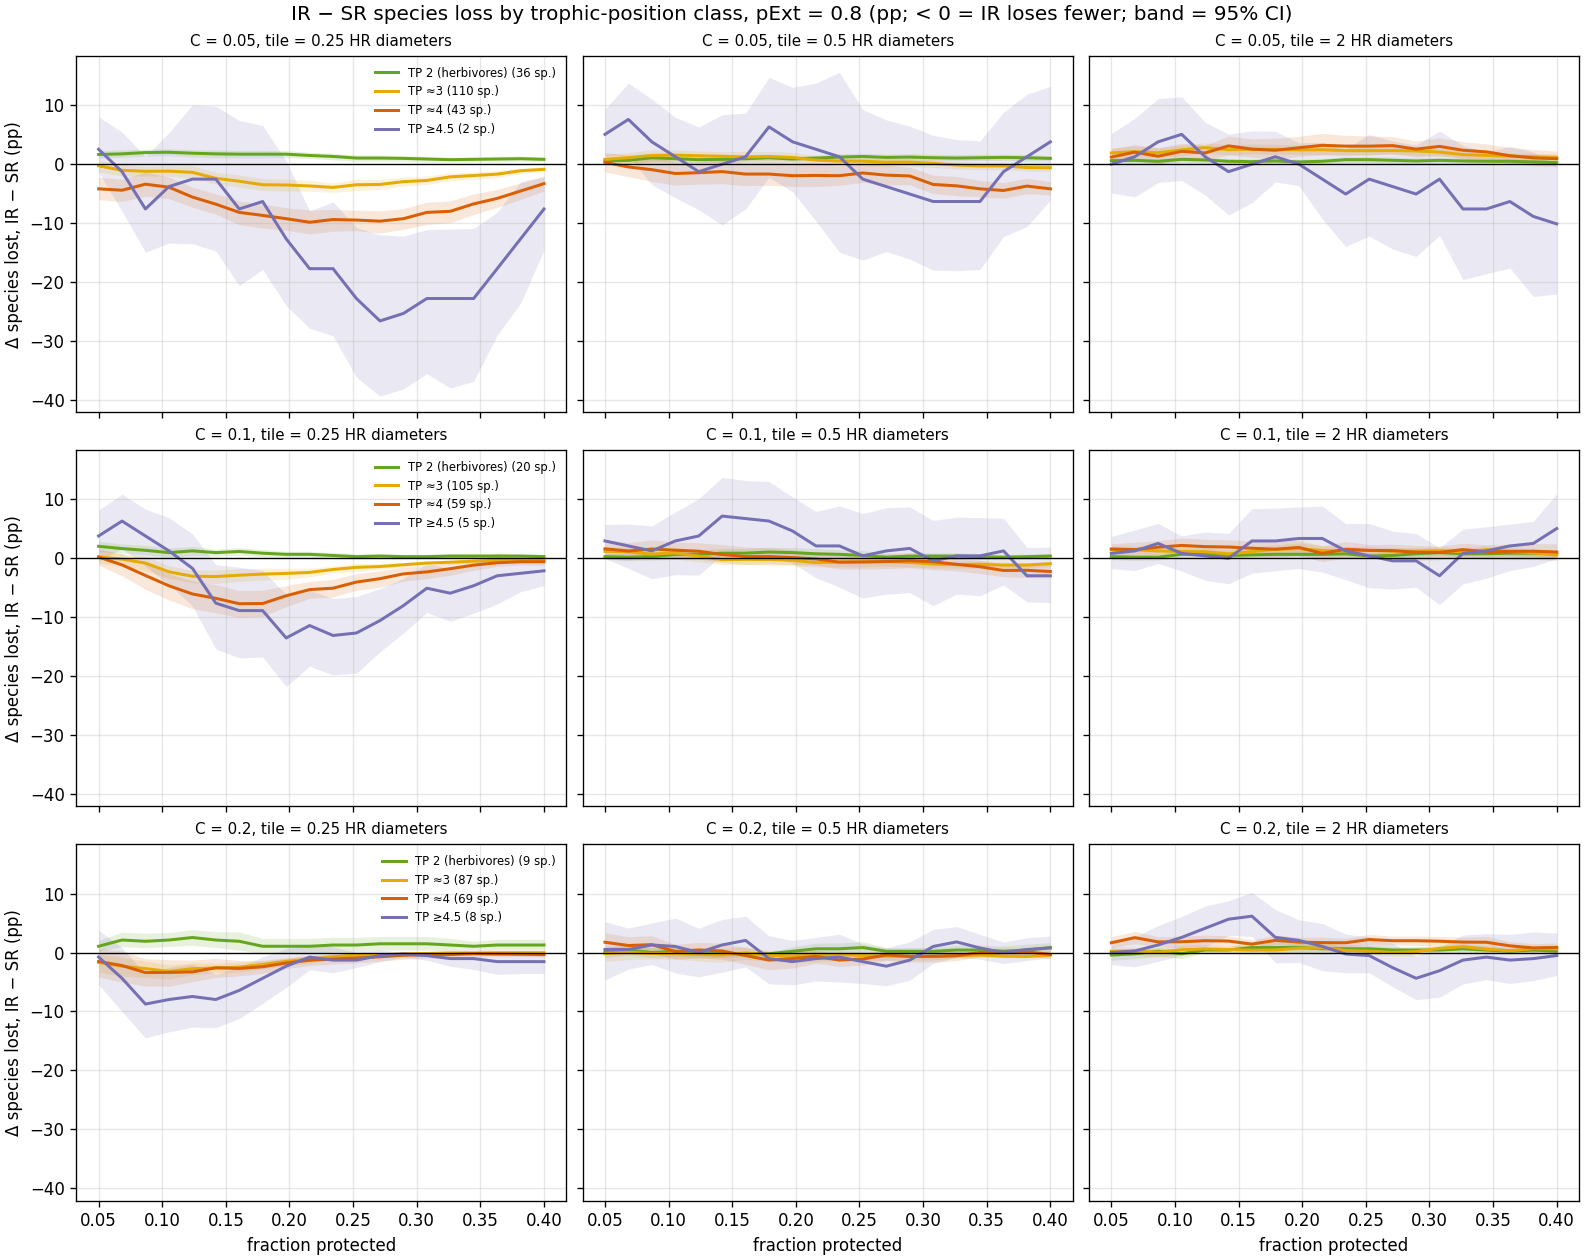
\includegraphics[width=0.9\textwidth]{loss_by_trophic_class_diff_pext0.8.png}
\caption{IR $-$ SR species loss by flow trophic-position class at $p_\text{ext}=0.8$. Existing figure
(\code{loss\_by\_trophic\_class.py}).}\label{fig:tp}
\end{figure}

\subsection{Three observations that are not in the existing write-ups}\label{sec:new}
\begin{enumerate}
\item \textbf{Grain changes absolute losses far more than the strategy does.} Averaged over the design, SR
loses 6.2\% of species with $t=0.25$ and 23.3\% with $t=8$ for the same protected area fraction (IR: 4.8\%
and 23.6\%). The strategy contrast is at most 1.4\pp{} on the same scale. Choosing where to protect at a
fine grain is worth an order of magnitude more than the choice of criterion.
\item \textbf{IR's interaction advantage is almost entirely direct.} At $t=0.25$, $-5.8$ of the $-6.3$\pp{}
arise in the primary-extinction phase, before any cascade. The species advantage is split about evenly
between primary ($-0.66$\pp) and secondary ($-0.77$\pp). The headline interaction result therefore depends
on \emph{which populations are shielded from primary extinction}, and only weakly on the cascade model.
\item \textbf{Population-level interaction loss tells the same story more strongly at fine grain}
($-7.2$\pp{} at $t=0.25$) and stays near $-1$\pp{} from $t=1$ upwards.
\end{enumerate}

%=====================================================================
\section{Assessment: strong points}

\begin{enumerate}
\item \textbf{A clear, non-obvious and conditional result.} ``It depends on grain, and here is the sign
change'' is more useful and more publishable than ``IR is better''. It also gives a single axis along which
synergy, trade-off and convergence are ordered.
\item \textbf{Paired design with common random numbers.} Strategies are compared on identical worlds with
coupled extinction draws. Effects of a fraction of a percentage point are resolved with 50 seeds.
\item \textbf{Exact reproducibility.} Stored rows are regenerated character for character by the current
code (Section~\ref{sec:verified}); the exporters replay the sweep and can verify themselves against it.
\item \textbf{A community that is not imposed.} The biomass pyramid, population sizes and the surviving
species emerge from an energy budget instead of being allocated. Trophic positions reach about 4--5
(counting plants), and persistence has an explicit energetic meaning.
\item \textbf{A mechanism, not only a contrast.} The population-level export shows \emph{what} each plan
protects, and the trophic-class sweep shows \emph{who} benefits. Few simulation studies of reserve
selection go this far.
\item \textbf{Documented design path.} The parameter document and the design document record why each choice
was made and which diagnostic supports it, including the choices that were rejected.
\item \textbf{Fast enough to extend.} About 5--7 runs per second on 20 threads; a sensitivity sweep on a new
parameter is a matter of hours.
\end{enumerate}

%=====================================================================
\section{Assessment: gaps and issues}

I separate issues that could change the conclusions from those that affect presentation or maintenance.
Table~\ref{tab:issues} summarises them; the text explains the ones that need it.

\begin{table}[!htb]
\caption{Issues by area. Severity refers to the risk for the article's main claim.}\label{tab:issues}
\small
\begin{tabularx}{\textwidth}{@{}p{0.5cm}L p{1.6cm} p{4.6cm}@{}}
\toprule
\# & Issue & Severity & Remedy \\
\midrule
\multicolumn{4}{@{}l}{\emph{Interpretation of the main result}}\\
1 & The ``IR wins on both'' regime uses tiles smaller than a home range & \sev{high} & Reframe or justify;
report tile size relative to home-range area \\
2 & SR is probably a weak comparator at fine grain (few distinct scores, many empty tiles) & \sev{high} &
Tile-score diagnostics; null and abundance strategies \\
3 & Greedy top-$k$ without complementarity for both strategies & \sev{high} & Run the complementarity
variants already in the code \\
4 & Result partly follows from herbivores being numerous and immune to starvation & medium & State it; test
with alternative basal treatment or weights \\
\multicolumn{4}{@{}l}{\emph{Model}}\\
5 & Primary extinction ignores population size and is spatially independent & \sev{high} & Size-dependent
and spatially correlated variants \\
6 & No sensitivity to $\rhobar$, home range, $B_0$, $n_{\min}$, TE & \sev{high} & Reduced sweeps \\
7 & Static, donor-controlled energetics; no dynamics or top-down effects & medium & State as scope \\
8 & Interaction metric is presence/absence at species level & medium & Add flux- or redundancy-weighted
metric \\
9 & Realised connectance is low (0.016--0.034) & low--medium & Compare with empirical webs in a supplement \\
10 & Protected-tile extinction probability hard-coded at 0.01 & low & Make it a parameter; one check \\
\multicolumn{4}{@{}l}{\emph{Statistics and design}}\\
11 & Pooled standard errors in the summary tables treat non-independent runs as independent & medium &
Cluster by seed (done in Table~\ref{tab:grain}) \\
12 & 1,080 cell tests with a 2-SE rule and no multiplicity control & low & Model-based analysis or FDR \\
13 & Budget truncation at coarse grain; zero tiles protected for $t=8$, $f<0.11$ & medium & Report
realised budgets; drop or redefine $t=8$ \\
14 & Two definitions of trophic level in the outputs & low & Use flow trophic position throughout \\
15 & Robustness shocks switched off in all current runs & low & Decide whether they belong in the paper \\
\multicolumn{4}{@{}l}{\emph{Engineering}}\\
16 & No unit tests; legacy models still inside \code{World.scala} behind string switches & medium &
Regression snapshot, then prune \\
17 & Build file carries OSGi and fat-JAR settings for discarded workflows; library version mismatch & low &
Simplify \code{build.sbt} \\
\bottomrule
\end{tabularx}
\end{table}

\subsection{Issues bearing on the main result}

\paragraph{1. The winning regime is below the scale of a home range.} The median home-range radius is 0.02,
so a median home range covers $\pi r^2\approx1.26\times10^{-3}$ of the landscape. A tile at $t=0.25$ has side
0.01 and area $10^{-4}$: one home range spans about 12.6 tiles. At $t=0.5$ it spans about 3.1 tiles; only
from $t=1$ is a tile larger than a home range. A population is nonetheless a point assigned to a single
tile, and protecting that tile protects the whole population. The two tile sizes at which IR is better on
both counts are therefore exactly the two at which a management unit is smaller than the area the organisms
use. A reviewer in conservation planning is likely to say that protecting a twelfth of a home range does not
protect a population. This does not invalidate the result, but it changes what it means. Two honest readings
are available: (a) fine tiles approximate \emph{population-level} targeting, and the result says that when
managers can target individual populations, an interaction criterion picks better ones; (b) the practical
range of the model is $t\geq1$, where the finding is a small trade-off. The article has to choose and argue
one of these, and I recommend showing how the result changes if protection is granted in proportion to the
fraction of the home range that is covered.

\paragraph{2. SR may be a weak comparator at fine grain.} At $t=0.25$ there are 10,000 tiles and
3,600--6,800 populations, clustered. At budget 0.15 the 1,500 tiles chosen by SR hold 2,556--3,497
populations, that is 1.7--2.3 populations per protected tile. A tile's species richness can then only take a
handful of small integer values, so SR must be choosing among large groups of tied tiles, and ties are
broken at random. The egocentric interaction score counts links to partners up to several tiles away and so
has many more distinct values. Part of IR's fine-grain advantage could therefore be ``a criterion with
resolution against a criterion without'', and not specifically ``interactions against species''. I have not
measured the tie structure directly (tile identities are not in the stored outputs); this is an inference
from the counts above and it needs checking. The check is cheap: record the distribution of tile scores per
strategy, and add three reference strategies that already exist in the code, namely random tiles, random
among occupied tiles, and abundance (most populations). If abundance or a tie-free variant of SR recovers
most of IR's gain, the story changes; if not, the result is much stronger for having survived the test.

\paragraph{3. No complementarity.} Real systematic conservation planning does not pick the richest sites;
it picks sites that complement each other. A richness-greedy SR is known to be inefficient, so beating it is
a lower bar than beating a complementarity-based species plan. Species- and interaction-complementarity
strategies exist in \code{ManagementLandscape} from earlier versions but have not been run on the current
model. This is the comparison reviewers will ask for first.

\paragraph{4. Herbivore dominance and immunity.} Herbivore populations are 63--79\% of all populations and
cannot starve. A criterion that counts species is drawn to tiles full of herbivore populations; a criterion
that counts interactions is drawn to consumers, each of which brings several links. Since consumers are the
only populations that can be lost secondarily, shifting protection towards them is bound to help. The
mechanism is real within the model, but its strength depends on two modelling choices (implicit plants, donor
control) that should be named as such in the paper.

\paragraph{5. Primary extinction.} Every population faces the same probability regardless of whether it has
10 or 10,000 individuals, and draws are independent across populations and tiles. Population sizes are now
an output of the model, so ignoring them is an inconsistency. Size-dependent extinction would favour
herbivores (large populations) and penalise top consumers further, which could either strengthen IR's
advantage (it protects the vulnerable ones) or change which populations are worth protecting. Real threats
are also spatially correlated, which interacts with the clustering of populations. Both variants are small
code changes and belong in the robustness section.

\paragraph{6. Untested assembly parameters.} The design document shows that $\rhobar$ moves richness from
about 110 to 225 species and links per species from 1.3 to 6.2. The grain result has only been obtained at
$\rhobar=0.03$ and one home-range size. Because the result is expressed in home-range units, its dependence
on home range and on population density per tile is the central robustness question.

\subsection{Statistics and design}\label{sec:stats}
\paragraph{11. Standard errors.} The summary tables report standard errors of about 0.03--0.05\pp{} for
the tile-size means. These are computed over all rows of a group, but the 360 design cells of one
connectance share the same 50 assembled worlds, so rows are not independent. Averaging within seed first
gives standard errors of 0.06--0.21\pp{} (Table~\ref{tab:grain}), two to four times larger. Every main
effect in Table~\ref{tab:grain} remains many standard errors from zero except the species contrast at
$t=0.5$ ($-0.24\pm0.11$), which should be described as marginal. The per-cell classification uses 50 seeds
within a cell and is not affected, but adjacent cells are correlated and there is no control for 1,080
simultaneous tests; a mixed model with seed as a random effect would be cleaner than counting significant
cells.

\paragraph{13. Budget discreteness.} Budgets are truncated to whole tiles. With nine tiles, any budget
below 0.111 protects nothing, which is why the first cells at $t=8$ are exactly zero; with 36 tiles the step
is 2.8\%. I suggest reporting realised budgets and treating $t=8$ as a boundary case outside the main
figures.

\paragraph{Saturation at fine grain.} Because most small tiles are empty, a budget defined as a fraction of
tiles covers a much larger fraction of populations (Table~\ref{tab:pops}). Above roughly 30\% both strategies
protect nearly every occupied tile. An alternative budget axis, the fraction of \emph{occupied} tiles or of
populations, would make grains comparable and would remove the artificial ties.

\subsection{Engineering}
The code is in better shape than the repository was. The remaining risks are that the paper model shares
\code{World.scala} with four superseded abundance models and three cascade rules, selected by strings, and
that there is no automated test. The hand-over guide's plan is sound: write a regression snapshot of the
paper configuration, then delete the unused branches and check that outputs are unchanged. I have not done
this, because the instruction for this task was to leave the code logic untouched. The build file sets the
fat-JAR main class to a runner that is now in the legacy folder, enables an OSGi plugin needed only by the
old OpenMOLE workflows, and declares \code{scala3-library} 3.1.0 alongside Scala 3.3.3.

%=====================================================================
\section{Towards an article}

\subsection{Proposed central claim}
\begin{quote}
\emph{Whether protecting interactions and protecting species are aligned depends on the grain of
management relative to the scale at which organisms use space. With fine-grained units, selecting sites by
the interactions they support retains more of the food web and no fewer species; with coarse units the two
criteria select similar sites and a small trade-off appears.}
\end{quote}
This framing has three advantages: it does not depend on IR ``winning''; it connects to an established
literature on scale in conservation planning; and it turns the weakest point (issue 1) into the subject of
the paper, provided the sub-home-range regime is treated openly.

\subsection{A possible storyline}
\begin{enumerate}
\item \textbf{Motivation.} Interactions can be lost before species; planning targets species. Proposals to
target interactions lack tests of when it matters.
\item \textbf{Model.} A spatial food web whose community is assembled by energy flow, so that who persists
after disturbance has a mechanistic basis.
\item \textbf{Result 1: grain orders the outcomes} (Table~\ref{tab:grain}, Figure~\ref{fig:heat}): synergy,
then trade-off, then convergence.
\item \textbf{Result 2: the two plans protect the same species but different populations}
(Table~\ref{tab:pops}): the interaction criterion shifts protection up the food web.
\item \textbf{Result 3: the benefit accrues to high trophic positions} (Figure~\ref{fig:tp}), at a small
cost to herbivores.
\item \textbf{Result 4: context.} Stronger pressure amplifies the contrast; denser webs damp it, consistent
with redundancy of links.
\item \textbf{Discussion.} What grain means in practice; why richness and interaction criteria converge
when units are large; what data would be needed to apply an interaction criterion; limits of a static
energetic model.
\end{enumerate}

\subsection{Candidate figures}
\begin{table}[H]
\small
\begin{tabularx}{\textwidth}{@{}p{1.2cm}L p{4.2cm}@{}}
\toprule
Figure & Content & Status \\
\midrule
1 & Model schematic: metaweb $\rightarrow$ ranges $\rightarrow$ population web $\rightarrow$ energy flow
$\rightarrow$ tiles and protection $\rightarrow$ extinction phases & to draw (the schematic in
\code{legacy/misc} describes something else) \\
2 & Loss against budget, SR and IR, three grains & exists (Fig.~\ref{fig:curves}); add species panel \\
3 & Contrast over grain $\times$ budget, species and interactions & exists (Fig.~\ref{fig:heat}); consider a
single ``phase diagram'' of synergy / trade-off / tie \\
4 & What is protected: populations by trophic position, overlap of plans & exists in parts; redraw from
Table~\ref{tab:pops} \\
5 & Loss by trophic class & exists (Fig.~\ref{fig:tp}) \\
S & Assembled-web realism; sensitivity to $\rhobar$, home range, $B_0$; foraging rules; reference and
complementarity strategies; size-dependent extinction & mostly to do \\
\bottomrule
\end{tabularx}
\end{table}

\subsection{Claims the current evidence does and does not support}
\begin{itemize}
\item \emph{Supported:} within this model and parameter set, IR loses fewer interactions than SR at every
grain; the species contrast changes sign with grain; the plans differ in the populations they protect; the
gain is concentrated at high trophic positions.
\item \emph{Not yet supported:} that the result holds for other community densities or home-range sizes;
that IR beats a complementarity-based species plan; that the fine-grain advantage is specific to
interactions and not to score resolution or abundance; any statement about real landscapes.
\item \emph{Do not reuse} conclusions from earlier model versions (``SR wins in 79\% of runs'', ``IR only
wins with coarse tiles''). The second is the opposite of the current result.
\end{itemize}

%=====================================================================
\section{Recommended next steps, in priority order}\label{sec:todo}

\begin{enumerate}
\item \textbf{Reference strategies on the current model} (issue 2 and 3): random, random among occupied
tiles, abundance, species complementarity, interaction complementarity; plus the distribution of tile
scores and number of ties per grain. Small code additions to the runner, no model change. This decides how
the main result should be worded.
\item \textbf{Decide how to treat sub-home-range tiles} (issue 1). At minimum a robustness run in which
protection is proportional to home-range coverage, or in which a population counts as protected only if
most of its home range is.
\item \textbf{Sensitivity of the grain result} to $\rhobar\in\{0.01,0.03,0.1\}$ and to median home range, on
a reduced design (three grains, a few budgets, $p_\text{ext}=0.8$).
\item \textbf{Extinction rule variants} (issue 5): probability decreasing with population size; spatially
correlated threat.
\item \textbf{A budget axis comparable across grains}: fraction of occupied tiles or of populations.
\item \textbf{Statistics}: seed-clustered errors everywhere; a mixed model for the grain $\times$ budget
$\times$ pressure $\times$ connectance effects.
\item \textbf{One trophic definition} in all outputs, and a flux-weighted interaction metric.
\item \textbf{Code}: paper-model regression snapshot, then removal of the superseded models and unused
strategies; a few unit tests on \code{EnergyFlow}.
\end{enumerate}
Items 1--3 could each overturn or sharpen the headline and should come before any writing of results.

%=====================================================================
\section{The repository after the clean-up}\label{sec:repo}

\begin{verbatim}
README.md                    overview, layout, quick start
build.sbt, project/          build
src/main/scala/econetcons/   current model, runners, checks (21 files)
analysis/                    README with commands; paper_sweep/ scripts; figures/
data/paper_sweep/            sweep, population export, trophic sweep, logs
data/emergent_design/        diagnostic runs behind the parameter choices
docs/                        MODEL_PARAMETERS, MODEL_DESIGN_AND_RESULTS,
                             ASSESSMENT_GUIDE, report/ (this document)
legacy/                      earlier versions, by period, with a README
\end{verbatim}

\paragraph{What changed.}
\begin{itemize}
\item About 90 output files, scripts and workflows of earlier model versions moved from the repository
root to \code{legacy/}, grouped by period so that each script sits next to the files it reads and writes.
\item Twenty Scala files of earlier versions (runners, diagnostics, probes) moved to \code{legacy/scala/}
and are no longer compiled. Nothing in the current code referred to them except in comments.
\item Design-evidence files moved to \code{data/emergent\_design/}; documentation moved to \code{docs/};
\code{biomass\_pyramid\_plan.md} renamed \code{MODEL\_DESIGN\_AND\_RESULTS.md}.
\item New or rewritten: root \code{README.md}, \code{legacy/README.md},
\code{data/emergent\_design/README.md}, \code{analysis/requirements.txt}; path references updated.
\item Git: bulky legacy outputs (about 110\,MB) are ignored and remain only on the original machine; editor
database files are no longer tracked.
\end{itemize}

\paragraph{What did not change.} No model, runner or analysis code was edited (the only edit outside
documentation is a two-line comment in \code{build.sbt}). No data file under \code{data/} or figure under
\code{analysis/figures/} was modified. The checks listed in Section~\ref{sec:verified} were run before and
after the move.

\paragraph{Things a new collaborator should know.}
\begin{itemize}
\item ``IR'' in current files is the egocentric variant; in legacy files the same label means the discarded
variant and today's IR is called EIR.
\item The legacy OpenMOLE workflows and the cluster fat-JAR no longer work without copying files back from
\code{legacy/scala/}.
\item Some design-evidence files were produced with intermediate code and cannot be regenerated; this is
noted in their README.
\item Spatial filtering of interactions (links absent because partners never meet) is a deliberate design
choice, not a bug.
\end{itemize}

\end{document}
